\documentclass[../main.tex]{subfiles}

\begin{document}
\section{Simulation}
\subsection{Numerical setup}\label{sec:numerical}
The 2D incompressible Navier Stokes equations are forced in a periodic domain of size $2\pi \times 2\pi$ with a forcing term that is located in a disk of radius $\pi/k_r$ centered at the origin. The range of values for the parameter $k_r$ is taken to be $\{8, 16, 32, 64\}$ and in all the cases the size of the vortices, which is controlled by $k_\ell$, is set to $k_\ell = 4 k_r$. The parameter $k_r$ being one of those values in the previous set represents how smaller is the perturbation region (in diameter) compared to the domain size ($2\pi$). The other parameter $k_\ell$ accounts for the number of vortices introduced in the domain, when there are no other vortices traveling in the domain. In those conditions, $(\pi k_\ell^2)/(\pi k_r^2) = 16$ vortices are introduced in the domain (see \cref{fig:forcing}).
\begin{figure}[ht]
	\centering
	\begin{subfigure}{0.49\textwidth}
		\centering
		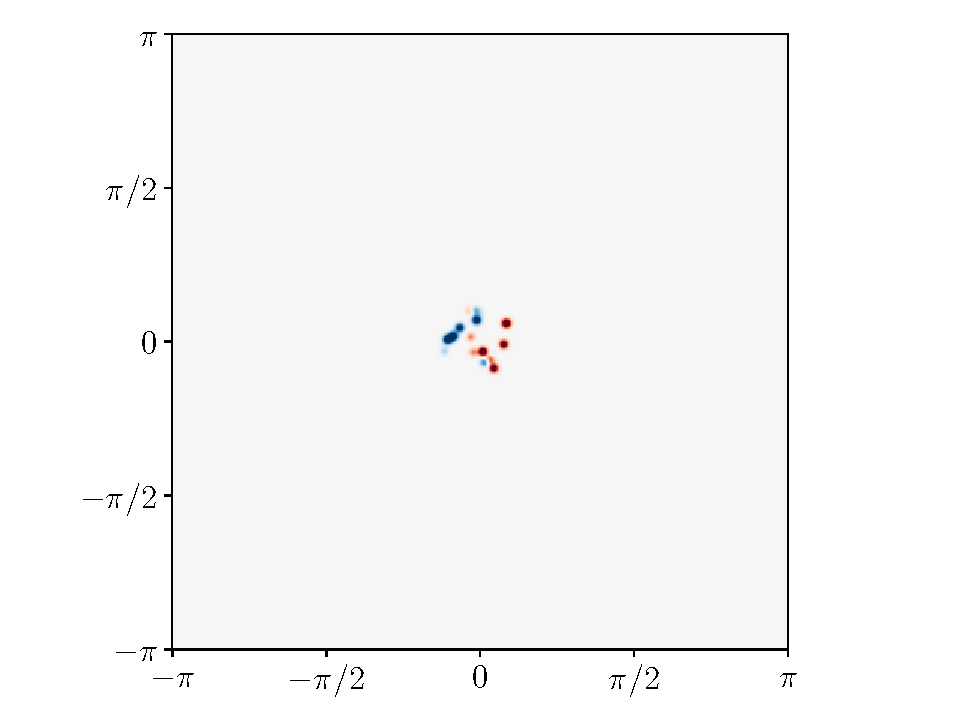
\includegraphics[width=\textwidth]{images/forcing32_8.pdf}
		\caption{$k_r = 8$}
	\end{subfigure}
	\begin{subfigure}{0.49\textwidth}
		\centering
		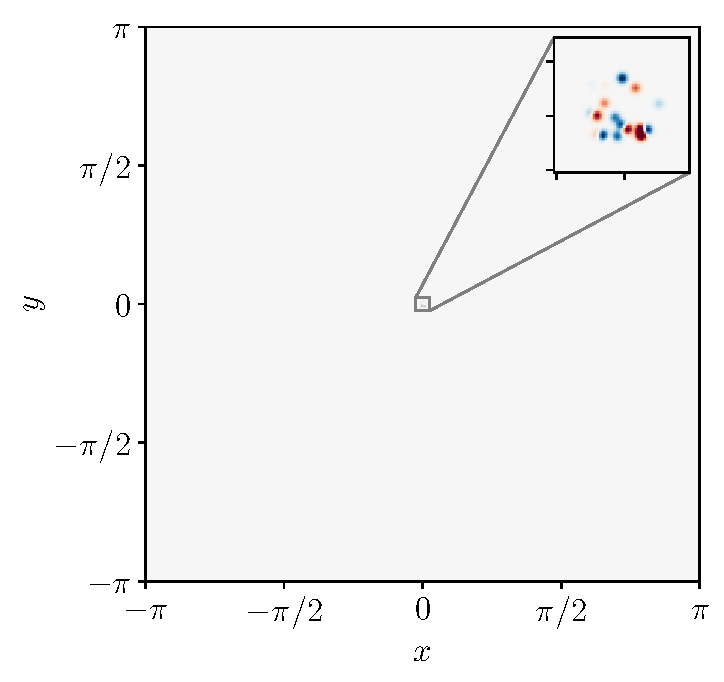
\includegraphics[width=\textwidth]{images/forcing32_64.pdf}
		\caption{$k_r = 64$}
	\end{subfigure}
	\caption{Forcing term for different values of $k_r$. Red colors and blue colors mean different direction of rotation for each vortex. The reader may notice that indeed the diameter of the forcing region is about 8 times smaller than the total size of the domain. In the second plot, this property is less noticeable, but it is still true, this case 64 times smaller.In the second plot, the colors have been enhanced to make the plot more clear.}
	\label{fig:forcing}
\end{figure}

The Reynolds number is the other parameter that plays an important role in the whole simulation. This project has simulated fluid flows for Reynolds numbers within the set $\{0.25, 0.5, 1, 2, 4, 8, 16, 32, 64, 128\}$, each of those requiring different resolution as we increase the Reynolds number.

A pseudo-spectral method has been used to solve the Navier Stokes equations, based on the Fourier basis and then using a 4th-order low-storage Runge-Kutta method to integrate the resulting ordinary differential equation. As explained in \cite{rungekutta}, this method differs from the conventional one in the . For more information, the reader is encouraged to read the article from \cite{rungekutta} or check the source codes in the link provided below.

The codes have been run in a cluster with 40 to 80 cores, owned by IDRIS\footnote{For more information about the resources they provide, check their website (accessed 19/06/2024): \url{http://www.idris.fr/}.} and MESOPSL\footnote{For more information about the resources they provide, check their website (accessed 19/06/2024): \url{https://wwwmesopsl-new.obspm.fr/}.}, depending on the simulation. Two different kinds of simulations have been performed: parallel simulations and embarrassingly parallel simulations. In the parallel simulations, the Fourier domain is divided among all the processors, allowing them to work simultaneously on different parts of the problem. In the embarrassingly parallel simulations, each simulation runs independently on a single core. Multiple simulations are executed concurrently, one on each available core, and the results are averaged afterward to obtain more accurate conclusions. Details about the parallelization of the code will not be delved into, but in brief... If the reader is interested in the details, the article from~\cite{mpi} is higly recommended. For the parallel code, a variable time step is used throughout the whole simulations in order to take into account the advection stability condition. For the embarrassingly parallel code, a fixed time step is used, in order to better compare the results between the different runs from the same simulation. The time step is chosen by eye after studying the evolution of the time steps during the parallel simulations. \cref{tab:simulations} shows the different simulations performed during the project as well as the resolution in physical space used in each case.
\begin{table}[ht]
	\centering
	\def\tickgreen{\textcolor{color_green3}{\ding{51}}}
	\def\tickblue{\textcolor{color_blue3}{\ding{51}}}
	% set space between columns
	\setlength{\tabcolsep}{5pt}
	% set space between rows
	\renewcommand{\arraystretch}{1.5}
	\begin{tabular}{c|cccccccccc}
		\diagbox[width=\dimexpr \textwidth/16+2\tabcolsep\relax, height=1cm]{$k_r$}{$\Re$} & 0.25             & 0.5              & 1                & 2                         & 4                          & 8                          & 16                         & 32                         & 64                & 128               \\
		\hline
		8                                                                                  & \tickgreen_{512} & \tickgreen_{512} & \tickgreen_{512} & \tickgreen\tickblue_{512} & \tickgreen\tickblue_{1024} & \tickgreen\tickblue_{1024} & \tickgreen\tickblue_{1024} & \tickgreen\tickblue_{2048} & \tickgreen_{2048} & \tickgreen_{4096} \\
		16                                                                                 &                  &                  &                  & \tickblue_{1024}          & \tickblue_{2048}           & \tickgreen\tickblue_{2048} & \tickgreen\tickblue_{2048} & \tickgreen\tickblue_{2048} & \tickgreen_{4096} & \tickgreen_{4096} \\
		32                                                                                 &                  &                  &                  & \tickblue_{2048}          & \tickblue_{4096}           & \tickgreen\tickblue_{4096} & \tickgreen\tickblue_{4096} & \tickgreen\tickblue_{4096} & \tickgreen_{8192} & \tickgreen_{8192} \\
		64                                                                                 &                  &                  &                  &                           &                            & \tickgreen_{8192}          & \tickgreen_{8192}          & \tickgreen_{8192}          &                   &                   \\
	\end{tabular}
	\caption{Simulations performed during the project varying the Reynolds number and the forcing parameter $k_r$. The green check mark symbols indicate the simulations done in parallel, splitting the domain between different cores. The blue check mark symbols indicate the simulations done in embarrassingly parallel, where each simulation is done in a single but in many cores at the same time in order to produce statistics results. In each cell, the number indicates the resolution in each dimension employed, which have been proved (a posteriori) to be enough to well-resolve the system.}
	\label{tab:simulations}
\end{table}

The reader may observe that the resolution increases both as the Reynolds number and the forcing parameter $k_r$ increase. For the former, the resolution is increased in order to resolve the smaller scales that appear in the system. For the latter, the resolution is increased to resolve the smaller perturbation region.

It is worth-noting that the resolution in Fourier space is not the same as the one in physical space.

All the codes and data used for the simulations are available in the following repository: \url{https://github.com/victorballester7/final-master-thesis} (accessed on June 30, 2024).

\subsection{Results}\label{sec:results}
\end{document}
